\chapter{Estado da Arte}

%Outros transmissores/receptores na literatura, CIs disponiveis, outras propostas comerciais

%Oi, é tipo docs sim haha
%show
%hahha

Na literatura, diversos estudos estão sendo realizados na área de ondas milimétricas, mais especificamente nas faixas de 28, 38, 60, 71-76 e 81-86 GHz, devido a suas altas taxas de transmissão, exigido para aplicações da quinta geração de redes de comunicação mobile (5G) \cite{8567053}.

Em comparação com as faixas de mais baixa frequência (1-10 GHz), a atenuação é maior em bandas de mais alta frequência devido a sua absorção em nível molecular e atmosférica, limitando o alcance dessas bandas \cite{ichkov2017potentials}, como pode ser visto na Figura \ref{atenuacao}. Entretanto, isso pode ser considerado uma vantagem para redes de curto alcance devido ao menor risco de interferência por outros dispositivos.

\begin{figure}[htbp]
    \centering
    %\captionsetup{justification=centering}
    \caption{Atenuação em ondas milimétricas}
    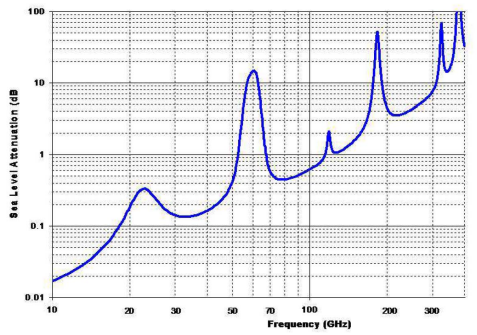
\includegraphics[width = \linewidth - 5cm]{atenuacao.png}
    
    \source{\citeauthor{8567053} (\citeyear{8567053})}
    \centering
    \label{atenuacao}
\end{figure}

Outro fator que difere as ondas milimétricas em relação as tradicionais é sua diretividade. Com a utilização de conjuntos de antenas, é possível criar um feixe mais estreito, criando um feixe mais diretivo. Devido ao menor tamanho de antena, é possível adicionar mais antenas em um mesmo espaço fixo, aumentando o ganho direcional em frequências mais altas, também resultando em menor interferência \cite{ichkov2017potentials}.

Para redes de área pessoal (\textit{WPAN - Wireless Personal Area Networks}), os principais trabalham se concentram na faixa de 60 GHz. Podem ser citados a camada de adaptação para envio de vídeos sem compressão \cite{7398126} e o desenvolvimento de um sistema de \textit{scheduling} para comunicação com ondas milimétricas levando em consideração métricas de qualidade de serviço (\textit{QoS - Quality of Service}) para aplicações de multimídia \cite{7010539}.

%CIs
Houve o desenvolvimento de alguns circuitos integrados (CI) capazes de realizar a transmissão e recepção de sinais na faixa de frequência de 60 GHz, como a Peraso\cite{Peraso}, GotMIC (Göteborg Microwave Integrated Circuits) \cite{gotmica}, Pasternack \cite{pasternack}, Infineon \cite{infineon}, Tensorcom \cite{tensorcom} e Analog Devices \cite{hmc6300}. 

Ao analisar critérios como preço, encapsulamento, dimensões, figura de ruído, ganho e, principalmente, documentação disponível, \citeauthor{TCC} optaram pela escolha da utilização dos CIs da Analog Devices para montagem do projeto.

%Propostas comerciais
Já existem produtos comercializados utilizando a frequência de 60 GHz, como sistemas de transmissão de vídeo sem compressão \cite{iogear} e roteadores de \textit{Wi-Fi} \cite{tplink}.

O estudo de sistemas utilizando ondas milimétricas está em destaque nos últimos anos, com o aumento da demanda de altas taxas de transferência sem fio devido ao 5G e a Internet das Coisas, \textit{Internet of Things (IoT)}. O desenvolvimento do método de fabricação todo feito no Brasil, o primeiro a ser produzido, possibilitará o avanço dos estudos nessa faixa de frequência.